% !TeX root = RJwrapper.tex
\title{VARshrink: An R Package for Shrinkage Estimation of High-Dimensional Vector Autoregressive Models}


\author{by Namgil Lee and Sung-Ho Kim}

\maketitle

\abstract{%
Vector autoregressive (VAR) models are widely used to study dynamic relationships in multivariate time series, with applications ranging from economic and financial forecasting to gene network analysis in systems biology and brain connectivity analysis in neuroscience. High-dimensional VAR models involve many parameters, increasing computational costs and making coefficient estimation more challenging. Shrinkage methods address these challenges by regularizing the coefficient estimates and improving their stability. We present the R package VARshrink, which provides ridge, nonparametric, fully Bayesian, and semiparametric shrinkage estimators through a unified interface. As its main design feature, VARshrink returns objects that inherit from classes in the widely used vars package, allowing existing methods for analysis, visualization, and forecasting to be reused. The package also supports model comparison using information criteria adapted to shrinkage estimation. We illustrate the main workflow with reproducible R code and compare the implemented estimators in numerical experiments.
}

\providecommand{\pandocbounded}[1]{#1}

\section{Introduction}\label{introduction}

Vector autoregressive (VAR) models describe the joint dynamics of
multiple time series through their lagged values. They are widely used
for macroeconomic forecasting and policy analysis, financial modeling,
the inference of gene regulatory networks from time-course data in
systems biology, and the analysis of dynamic brain connectivity in
neuroscience
\citep{Hamilton94, Koop10BayesianVAR, Rhein07c, Harrison03}. However, the
number of parameters increases rapidly with both the number of variables
and the lag order. High-dimensional VAR models can therefore be
computationally demanding and difficult to estimate reliably.
Shrinkage methods address these challenges by regularizing coefficient
estimates, thereby improving estimation stability and potentially
forecasting performance.

Several \textbf{R} packages provide methods for VAR and related multivariate
time-series models. The \pkg{MTS} package provides tools for VAR,
VARMA, seasonal VARMA, and other multivariate time-series models
\citep{Tsay18}, while
\CRANpkg{vars} supports estimation, inference, forecasting, and
diagnostic analysis for VAR, SVAR, and SVEC models \citep{Pfaff18}. For
large systems, \CRANpkg{BigVAR} estimates VAR and VARX models using
structured penalties \citep{Nicholson2026BigVAR}, whereas
\CRANpkg{bigtime} estimates sparse VAR, VARX, and VARMA models using
structured lasso penalties \citep{Wilms2023bigtime}.

Several packages also support Bayesian VAR analysis.
\CRANpkg{bvartools} assists in setting up Bayesian inference for VAR
and vector error-correction models \citep{Mohr2024bvartools}.
\CRANpkg{bayesianVARs} implements MCMC estimation of Bayesian VARs with
shrinkage priors and stochastic volatility
\citep{Gruber2026bayesianVARs}, while \CRANpkg{bvarsv} implements
time-varying parameter VARs with stochastic volatility
\citep{Primiceri2005timevarying, Krueger2015bvarsv}. \CRANpkg{BVAR}
implements hierarchical prior selection for conjugate priors following
\citeauthor{Giannone2015prior} \citetext{\citeyear{Giannone2015prior}; \citealp{KuschnigVashold2021BVAR}}.
\CRANpkg{bsvarSIGNs} uses Minnesota and dummy-observation priors with
estimated hyperparameters in structural VARs identified by sign, zero,
and narrative restrictions \citep{WangWozniak2025bsvarSIGNs}.

In this study, we focus on shrinkage estimation of VAR model parameters.
Shrinkage estimation methods have played crucial roles in
high-dimensional statistical modeling
\citep{LedoitWolf2004shrinkcov, Bohm2009shrinkage, Fiecas2011aoas, Beltra2013shrinkageEEG}. For VAR
models, an extensive literature has developed on regularization and
shrinkage priors, including Minnesota-type priors and more recent
global-local shrinkage priors. Frequentist penalized estimation has
also been widely studied. Approaches directly related to this package include
a Stein-type nonparametric shrinkage estimation method \citep{Rhein07c},
Bayesian VARs using informative priors
\citep{Doan84, Litterman86, Banbura10, Koop10BayesianVAR}, Bayesian VARs
using noninformative priors \citep{Sun04, Ni05}, and a semiparametric
Bayesian approach adopting a modified \(K\)-fold cross-validation
\citep{LeeChoiKim2016}.

Shrinkage methods developed for purposes other than
multivariate time series analysis can also be applied to the estimation of
VAR parameters. For instance, the function \texttt{cov.shrink()} in the package \CRANpkg{corpcor} was developed
to compute shrinkage estimates of covariances, but
it has also been used to estimate VAR coefficients
\citep{Rhein07c, Schafer17}. Moreover, VAR models can be reformulated as multivariate regression problems, allowing penalized least squares methods to be used for
shrinkage estimation of VAR parameters. Examples include the functions
\texttt{lm.gls()} for generalized least squares and \texttt{lm.ridge()} for
ridge regression in the package \CRANpkg{MASS} \citep{Ripley18}; the
function \texttt{glmnet()} for Lasso and Elastic-Net regularized
generalized linear models in the package \pkg{glmnet}
\citep{Frideman18}; the function \texttt{linearRidge()} for ridge
regression in the package \pkg{ridge} \citep{Moritz18}.

While Bayesian approaches have been widely used in the literature,
nonparametric and semiparametric approaches have advantages
for high-dimensional VARs with several hundred or more
time series variables due to their relatively low computational cost
\citep{Rhein07c}. In contrast,
Bayesian approaches can flexibly impose proper assumptions on multivariate
time series data, such as VAR roots near unity and correlations
among noise processes \citep{LeeChoiKim2016}. In this sense, a
semiparametric approach serves as a trade-off between nonparametric and
parametric approaches \citep{LeeChoiKim2016}.

The main design contribution of \CRANpkg{VARshrink} is to extend the
workflow of \CRANpkg{vars} from ordinary least squares to shrinkage
estimation. Users can apply familiar methods from \CRANpkg{vars},
including ARCH-LM tests, causality analysis, diagnostic plots,
forecasting, impulse response analysis, and
forecast error variance decomposition, directly to
\textbf{R} objects obtained via shrinkage estimation methods in
\CRANpkg{VARshrink}. This compatibility also allows shrinkage
methods to be introduced within established applied and teaching
workflows based on \CRANpkg{vars}.

Relative to existing implementations, \CRANpkg{VARshrink} brings
together ridge regression, a Stein-type nonparametric estimator, fully
Bayesian estimation, and semiparametric Bayesian estimation in one
interface. Its fully Bayesian method includes both a natural conjugate
normal-Wishart prior and a non-conjugate
shrinkage-reference prior, with scale-mixture likelihoods available for
robust estimation. The package also provides likelihood and information
criterion methods that account for the selected noise distribution and
the effective number of parameters. These features are intended to
complement packages specializing in structured
penalties, hierarchical Bayesian prior selection, stochastic
volatility, or structural identification.

This paper is organized as follows. In Section 2, we
formulate VAR models as a multivariate regression
problem, which simplifies the implementation of the package.
We also describe the general distributional assumptions for the noise term
within a Bayesian framework.
Closed-form expressions for the shrinkage estimators implemented in the package are presented to clarify the role of the shrinkage intensity parameters in each method.
In addition, we explain how the effective
number of parameters is computed for shrinkage estimators.
Section 3 introduces the common interface function and provides sample code snippets to demonstrate the usefulness of the package.
In Section 4, we present numerical experiments using benchmark and
simulated data to compare the performance of the shrinkage estimation
methods. Discussion and conclusions are given in Sections 5 and 6.

\section{Models}\label{models}

\subsection{Multivariate linear regression formulation}\label{multivariate-linear-regression-formulation}

Let \(\mathbf{y}_t = (y_{t1},y_{t2},\ldots,y_{tK})^\top\) denote a
\(K\times 1\) vector of endogenous variables. A VAR model of order
\(p\) can be expressed as
\begin{equation}
    \mathbf{y}_t = \mathbf{A}_1 \mathbf{y}_{t-1} + \cdots + \mathbf{A}_p \mathbf{y}_{t-p} + \mathbf{C} \mathbf{d}_t + \boldsymbol\epsilon_t,
    \label{eq:VAReqnA}
\end{equation}
where \(\mathbf{d}_t\) is an \(L\times 1\) vector of deterministic
regressors, \(\boldsymbol\epsilon_t\) is a \(K\times 1\) noise vector,
and \(\mathbf{A}_1,\ldots,\mathbf{A}_p\) and \(\mathbf{C}\) are
coefficient matrices \citep{Hamilton94, Tsay05}.

The model equation \eqref{eq:VAReqnA} can be expressed in the
matrix form of a multivariate regression as
\begin{equation}
    \mathbf{Y} = \mathbf{X} \boldsymbol\Psi + \mathbf{E} \in \mathbb{R}^{N \times K},
    \label{eq:VAReqnMat}
\end{equation}
where
\(\boldsymbol\Psi = (\mathbf{A}_1, \mathbf{A}_2, \ldots, \mathbf{A}_p, \mathbf{C})^\top\)
is a \((Kp + L) \times K\) matrix of coefficients,
\begin{equation}
    \begin{split}
    \mathbf{Y} &= ( \mathbf{y}_{p+1}, \mathbf{y}_{p+2}, \ldots, \mathbf{y}_{T} )^\top \in \mathbb{R}^{N \times K},
    \\
    \mathbf{X} &= ( \mathbf{x}_{p+1}, \mathbf{x}_{p+2}, \ldots, \mathbf{x}_{T} )^\top \in \mathbb{R}^{N \times (Kp + L)}
    \end{split}
\end{equation}
are data matrices with
\(\mathbf{x}_t = (\mathbf{y}_{t-1}^\top, \ldots, \mathbf{y}_{t-p}^\top, \mathbf{d}_t^\top)^\top \in \mathbb{R}^{Kp + L}\),
\(\mathbf{E} = (\boldsymbol\epsilon_{p+1}, \ldots, \boldsymbol\epsilon_T)^\top\),
and \(N = T-p\).

\subsection{Mathematical expressions for shrinkage estimators}\label{mathematical-expressions-for-shrinkage-estimators}

In version 0.5 of the \textbf{R} package \CRANpkg{VARshrink}, ordinary
least squares (OLS) and five shrinkage estimation methods are
implemented: multivariate ridge regression \citep{Hoerl70, Golub79, Ripley18},
a Stein-type nonparametric shrinkage method \citep{Schafer05b, Rhein07c, Schafer17},
a full Bayesian shrinkage method \citep{Sun04, Ni05}, and two semiparametric
Bayesian shrinkage methods based on parameterized and K-fold
cross-validation, respectively \citep{LeeChoiKim2016}. OLS is included as a
baseline for settings in which the VAR is estimable without shrinkage.
For each shrinkage estimation method, the shrinkage estimator of the
coefficient matrix \(\boldsymbol\Psi\) takes a distinct mathematical form.

\subsubsection{(1) Multivariate ridge regression}\label{multivariate-ridge-regression}

The ridge regression estimator,
\(\widehat{ \boldsymbol\Psi }^\text{R} (\lambda)\), can be expressed in a
closed form as follows \citep{Hoerl70}:
\begin{equation}
    \widehat{ \boldsymbol\Psi }^\text{R} (\lambda) =
    \left( \mathbf{X}^\top \mathbf{X} + N \lambda \mathbf{I} \right)^{-1} \mathbf{X}^\top \mathbf{Y},
    \end{equation}
where \(\lambda \geq 0\) is called the regularization parameter or the
shrinkage parameter.

\subsubsection{(2) Stein-type nonparametric shrinkage method}\label{stein-type-nonparametric-shrinkage-method}

Suppose that the VAR model does not include a constant term, that is, a regressor whose value remains constant over time (e.g., \(d_t = 1\)).
Assuming that the data matrices \(\mathbf{X}\) and \(\mathbf{Y}\) have been mean-corrected,
let \(\mathbf{S}_\text{XX} = (N - 1)^{-1} \mathbf{X}^\top \mathbf{X}\),
\(\mathbf{S}_\text{XY} = (N - 1)^{-1} \mathbf{X}^\top \mathbf{Y}\), and
\(\mathbf{S}_\text{YY} = (N - 1)^{-1} \mathbf{Y}^\top \mathbf{Y}\) denote the sample covariance matrices, \(\mathbf{D}_\text{X} = \text{diag}(\mathbf{S}_\text{XX})\) and \(\mathbf{D}_\text{Y} = \text{diag}(\mathbf{S}_\text{YY})\) denote the diagonal matrices of sample variances, and \(\mathbf{R}_\text{XX}\), \(\mathbf{R}_\text{XY}\), and \(\mathbf{R}_\text{YY}\) denote the sample correlation matrices.
The shrinkage estimators of the correlation matrices are defined as:
\begin{equation}
    \widehat{\mathbf{R}}_\text{XX} =
    (1-\lambda) \mathbf{R}_\text{XX} + \lambda \mathbf{I}
    ,
    \qquad
    \widehat{\mathbf{R}}_\text{XY} =
    (1-\lambda) \mathbf{R}_\text{XY},
\end{equation}
where \(0 \leq \lambda \leq 1\) is the shrinkage parameter for the correlations.
And the shrinkage estimators of the variance matrices are defined as:
\begin{equation}
    \widehat{\mathbf{D}}_\text{X} = 
    (1-\lambda_v) \mathbf{D}_\text{X}  +
    \lambda_v s_\text{med} \mathbf{I},
    \ \ \widehat{\mathbf{D}}_\text{Y} =
        (1-\lambda_v) \mathbf{D}_{\text{Y}} +
    \lambda_v s_\text{med} \mathbf{I},
\end{equation}
where \(0 \leq \lambda_v \leq 1\) is the shrinkage parameter for the variances,
and \(s_\text{med}\) is the median of all sample variances.

The nonparametric shrinkage (NS) estimator of \(\boldsymbol\Psi\) can be expressed as follows \citep{Schafer05b, Rhein07c}:
\begin{equation}
    \widehat{ \boldsymbol\Psi }^\text{N} (\lambda, \lambda_v) =
    \widehat{\mathbf{D}}_\text{X}^{-1/2}
    \widehat{\mathbf{R}}_\text{XX}^{-1}
    \widehat{\mathbf{R}}_\text{XY}
    \widehat{\mathbf{D}}_\text{Y}^{1/2}.
\end{equation}
The shrinkage estimate \(\widehat{ \boldsymbol\Psi }^\text{N} (\lambda, \lambda_v)\) approaches the ordinary least squares estimate, \(\widehat{\boldsymbol\Psi}^{\text{OLS}} = \mathbf{S}_\text{XX}^{-1} \mathbf{S}_\text{XY}\), as \(\lambda\) and \(\lambda_v\) approach zero.

\subsubsection{(3) Full Bayesian shrinkage method}\label{full-bayesian-shrinkage-method}

The full Bayesian shrinkage method supports several likelihood and prior
specifications.

\paragraph{Likelihoods}\label{likelihoods}

We assume that the noise vectors are independent and identically distributed from a scale mixture of
multivariate normal distributions, including multivariate normal
distributions, multivariate t-distributions \citep{Ni05}, and
multivariate Laplace distributions (MLD) \citep{Eltoft06}. By
incorporating scale mixture distributions in the model assumption, we
can handle outliers appropriately and produce robust estimates
\citep{West84}. In specific, we consider that a noise vector can be
expressed as a product
\begin{equation}
    \boldsymbol\epsilon_t = \mathbf{z}_t q_t^{-1/2},
    \label{eq:productZD}
    \end{equation} where
\(\mathbf{z}_t \sim \text{N}_K(\mathbf{0}, \mathbf{\Sigma})\) is a
\(K\times 1\) vector having a multivariate normal distribution with the
mean vector of zeros and the covariance matrix of \(\boldsymbol\Sigma\),
and \(q_t \sim \text{Gamma}(\nu/2, \nu/2)\) is a random variable having
a gamma distribution with shape \(\alpha = \nu/2\) and rate
\(\beta = \nu/2\).
The \(\boldsymbol\epsilon\) has a multivariate t-distribution with degrees of freedom \(\nu\) when \(1<\nu<\infty\), a multivariate normal
distribution as \(\nu \rightarrow \infty\), and
a multivariate Cauchy distribution when \(\nu = 1\).
More detailed discussions can be found in the package vignette and \citet{LeeChoiKim2016}.

\paragraph{Conjugate prior}\label{conjugate-prior}

Let \(\boldsymbol\psi = \text{vec}(\boldsymbol\Psi) \in\mathbb{R}^{J}\) denote
the vectorized form of \(\boldsymbol\Psi \in\mathbb{R}^{(Kp + L)\times K}\), where
\(J = K (Kp + L)\).
The natural conjugate prior implemented in \CRANpkg{VARshrink} is a
normal-Wishart prior. Conditional on \(\mathbf{\Sigma}\), the
prior for \(\boldsymbol\psi\) is
\begin{equation}
  ( \boldsymbol\psi | \mathbf{\Sigma}, \delta )  
  \sim \text{N}_{J} \left( \mathbf{0}, \delta \mathbf{\Sigma} \otimes \mathbf{I} \right),
\end{equation}
where \(\otimes\) represents the Kronecker product of two matrices and \(\delta \equiv 1 / \lambda > 0\) is a reciprocal of a shrinkage parameter \(\lambda > 0\),
and an inverse Wishart distribution with a positive definite scale matrix \(\mathbf{L}_0\) and degrees of freedom \(m_0 > K - 1\) for \(\mathbf{\Sigma}\) as
\begin{equation}
  ( \mathbf{\Sigma} | \mathbf{L}_0, m_0 )
  \sim \text{InvWishart}\left(\mathbf{L}_0, m_0\right).
\end{equation}
The prior distributions for \(\delta\) and \(w = \nu / 2\) are given by
\begin{equation}
  \begin{split}
  \pi(\delta) & \propto 1, \\
  w & \sim \text{Gamma}(a_0, b_0),
  \end{split}
\end{equation}
for some \(a_0, b_0 > 0\).

\CRANpkg{VARshrink} uses a Gibbs MCMC method to sample
\((\boldsymbol\psi, \mathbf{Q}, \mathbf{\Sigma}, w, \delta)\)
from the conditional posterior distributions;
see the package vignette for more details.
Let \(\mathbf{Q} = \text{diag}(q_{p+1}, \ldots, q_T)\).
With \(\lambda \equiv 1 / \delta\), the mean of the conditional posterior distribution of \(\boldsymbol\psi\) given \((\mathbf{Q}, \mathbf{\Sigma}, w, \delta ; \mathbf{Y} )\) can be written as
\begin{equation}
  \widehat{\mathbf\Psi}^\text{F}_\text{CJ}( \lambda ) 
  =  \left( \mathbf{X}^\top \mathbf{Q} \mathbf{X} + \lambda \mathbf{I} \right)^{-1} \mathbf{X}^\top \mathbf{Q} \mathbf{Y}.
  \label{eq:expr-fbayes-cj-psihat}
\end{equation}

\paragraph{Non-conjugate priors}\label{non-conjugate-priors}

The non-conjugate prior adopted in \textbf{VARshrink} is the shrinkage-reference prior of \citet{Ni05}, which is given by
\begin{equation}
\begin{split}
  ( \boldsymbol\psi | \delta )
  & \sim \text{N}_{J} \left( \mathbf{0}, \delta \mathbf{I} \right),
  \\
  \pi( \mathbf{\Sigma} )
  & \propto |\mathbf{\Sigma}|^{-1} \prod_{1\leq i < j\leq K} (\lambda_i - \lambda_j)^{-1}, 
  \\
  \pi(\delta) & \propto 1, \\
  w & \sim \text{Gamma}(a_0, b_0),
\end{split}
\end{equation}
where
\(\lambda_1 > \lambda_2 > \cdots > \lambda_K\) are eigenvalues of \(\mathbf{\Sigma}\),
\(w = \nu / 2\), and \(a_0, b_0 > 0\).

With \(\lambda \equiv 1 / \delta\), the mean of the conditional posterior distribution of \(\boldsymbol\psi\) given \((\mathbf{Q}, \mathbf{\Sigma}, w, \delta; \mathbf{Y})\)
is given by
\begin{equation}
    \widehat{\boldsymbol\psi}^\text{F}_\text{NCJ}(\lambda)  = \left(\mathbf{\Sigma}^{-1} \otimes \left( \mathbf{X}^\top \mathbf{Q} \mathbf{X} \right) + \lambda \mathbf{I}_J     \right)^{-1} \text{vec}\left( \mathbf{X}^\top \mathbf{Q} \mathbf{Y} \mathbf{\Sigma}^{-1} \right).
    \label{eq:expr-fbayes-ncj-psihat}
\end{equation}

\subsubsection{(4) Semi-parametric shrinkage method}\label{semi-parametric-shrinkage-method}

In contrast to the full Bayesian approach, the semiparametric Bayesian approach selects the shrinkage parameter \(0 \leq \lambda < 1\) through parameterized cross-validation \citep{LeeChoiKim2016}.
Once the \(\lambda\) is fixed, the parameters \(\boldsymbol\psi\), \(\mathbf{\Sigma}\), and \(\mathbf{Q}\) are estimated at the mode of the marginal posterior density
\(\pi (\boldsymbol\psi, \mathbf{\Sigma} | \lambda; \mathbf{Y})\). In the
case of a non-conjugate prior for \(\boldsymbol\psi\) \citep{LeeChoiKim2016}, the mode
\(\widehat{\boldsymbol\psi}^\text{S} (\lambda)\)
is given by
\begin{equation}
    \widehat{\boldsymbol\psi}^{\text{S}} (\lambda)  =
    \left[\left(  \mathbf{\Sigma}^{-1} \otimes
          \left( \mathbf{X}^\top \mathbf{Q} \mathbf{X} \right) \right) + \frac{ (N - 1) \lambda}{1-\lambda} \mathbf{I}_J     \right]^{-1}
    \text{vec}\left( \mathbf{X}^\top \mathbf{Q} \mathbf{Y} \mathbf{\Sigma}^{-1} \right)
    .
    \label{eq:expr-sbayes-psihat}
\end{equation}
The covariance matrix \(\mathbf{\Sigma}\) is estimated in the same manner.

\subsection{Estimation of the effective number of parameters}\label{estimation-of-the-effective-number-of-parameters}

Although all shrinkage estimators are expressed in slightly different forms, they approach the ordinary least squares estimator (or the maximum likelihood estimator) as the shrinkage parameters decrease to zero, and they are shrunk toward zeros as the shrinkage parameters increase.
It implies that the effective number of parameters underlying a shrinkage estimator is controlled by the shrinkage parameter values.

The shrinkage estimators presented in the previous section can be expressed in a general form:
\begin{equation}
    \widehat{\boldsymbol\psi} (\lambda_0)  = \left[\left(\mathbf{\Sigma}^{-1} \otimes \left( \mathbf{X}^\top \mathbf{Q} \mathbf{X} \right) \right) + \lambda_0 \mathbf{I}_J     \right]^{-1} \text{vec}\left( \mathbf{X}^\top \mathbf{Q} \mathbf{Y} \mathbf{\Sigma}^{-1} \right),
    \label{eq:expr-phat-general}
\end{equation}
where \(\lambda_0 > 0\) is the shrinkage parameter.
A noise covariance matrix is approximated by its diagonal elements as \(\mathbf{\Sigma} \approx \mathbf{D}_\text{e} \equiv \text{diag}(\mathbf{\Sigma}) = \text{diag}(\sigma_{11}, \ldots, \sigma_{KK})\) to simplify the expression for \(\widehat{\boldsymbol\psi} (\lambda_0)\) as:
\[
  \widehat{\boldsymbol\psi} (\lambda_0)  
      \approx 
      \left[\left(\mathbf{I}_K \otimes \left( \mathbf{X}^\top \mathbf{Q} \mathbf{X} \right) \right) + \lambda_0 \mathbf{D}_\text{e} \otimes \mathbf{I}_{J/K}   \right]^{-1} \text{vec}\left(\mathbf{X}^\top \mathbf{Q} \mathbf{Y} \right),
  \]
or equivalently, for each \(j=1,2,\ldots,K\),
\begin{equation}
   \widehat{\boldsymbol\psi}_j (\lambda_0)
   \approx
    \left( \mathbf{X}^\top \mathbf{Q} \mathbf{X} + \lambda_0 \sigma_{jj} \mathbf{I}_{J/K} \right)^{-1} 
    \mathbf{X}^\top \mathbf{Q} \mathbf{y}_j
    ,
    \label{eq:expr-phat-general001}
\end{equation}
where \(\widehat{\boldsymbol\psi}_j (\lambda_0)\) and \(\mathbf{y}_j\) are the \(j\)th column vectors of \(\widehat{\boldsymbol\Psi} (\lambda_0)\) and \(\mathbf{Y}\).

From the definition of a hat matrix, \(\mathbf{H}(j, \lambda_0)\), we have \(\widehat{\mathbf{y}}_j \equiv \mathbf{H}(j, \lambda_0) \mathbf{y}_j = \mathbf{X} \widehat{\boldsymbol\psi}_j(\lambda_0)\),
and the hat matrix can be expressed as: \(\mathbf{H}(j, \lambda_0) \equiv
  \mathbf{X} \left( \mathbf{X}^\top \mathbf{Q} \mathbf{X} + \lambda_0 \sigma_{jj} \mathbf{I}_{J/K} \right)^{-1} \mathbf{X}^\top \mathbf{Q}.\)
Let \(\mathbf{X}^\top \mathbf{Q} \mathbf{X} = \mathbf{P} \mathbf{L} \mathbf{P}^\top\) denote the eigenvalue decomposition of \(\mathbf{X}^\top \mathbf{Q} \mathbf{X}\), where \(\mathbf{L} = \text{diag}(l_{11}, l_{22}, \ldots)\) is the diagonal matrix of eigenvalues.
The effective number of parameters, \(\kappa_\text{eff}\), is computed by the trace of the hat matrix as:
\begin{equation}
\kappa_\text{eff} (\lambda_0) = \sum_{j=1}^K \text{tr}\left( \mathbf{H}(j, \lambda_0) \right) = \sum_{j=1}^K \text{tr}\left( \left(\mathbf{L} + \lambda_0 \sigma_{jj} \mathbf{I}_{J/K} \right)^{-1} \mathbf{L} \right) = \sum_{j=1}^K \sum_{i=1}^{J/K} \frac{l_{ii}}{l_{ii} + \lambda_0 \sigma_{jj}}.
\end{equation}

With the estimated value for the effective number of parameters, the AIC and BIC values can be calculated as:
\begin{equation}
\begin{split}
\text{AIC}(\lambda_0) &= -2 \text{logLik} (\lambda_0) + 2 \kappa_\text{eff} (\lambda_0), \\
\text{BIC}(\lambda_0) &= -2 \text{logLik} (\lambda_0) + \kappa_\text{eff} (\lambda_0) \log(N),
\end{split}
\end{equation}
where \(\text{logLik}\) represents the log-likelihood.
We can use the AIC and BIC values to select an optimal value of the lag order, \(p\).

\section{Overview of the package}\label{overview-of-the-package}

The \textbf{R} package \CRANpkg{VARshrink} performs shrinkage estimation of the VAR model
coefficients \(\boldsymbol\Psi\) in \eqref{eq:VAReqnMat}
from multivariate time series data \(\mathbf{y}_1, \mathbf{y}_2,\) \(\ldots, \mathbf{y}_T \in \mathbb{R}^K\).
It estimates the so-called shrinkage intensity parameter \(\lambda > 0\), whose interpretation slightly differs across shrinkage estimation methods. Depending on the method, additional model parameters may also be estimated, such as the \(K\times K\) covariance matrix \(\mathbf{\Sigma}\) of the noise vector \(\boldsymbol\epsilon_t \in \mathbb{R}^K\) in \eqref{eq:productZD}.

\subsection{Package architecture}\label{package-architecture}

The software architecture of \CRANpkg{VARshrink} is illustrated in Figure \ref{fig:architecture}. The main interface function, \texttt{VARshrink()}, receives multivariate time series data in a \(T\times K\) matrix form, and outputs the estimated parameters as an instance of the \texttt{varshrinkest} class.
An instance of this class can then be used to produce useful time series analysis results through various class methods and analysis functions. Table \ref{tab:methods-pdf} summarizes the structure of \CRANpkg{VARshrink}, listing the available class methods and analysis functions.

\begin{figure}

{\centering 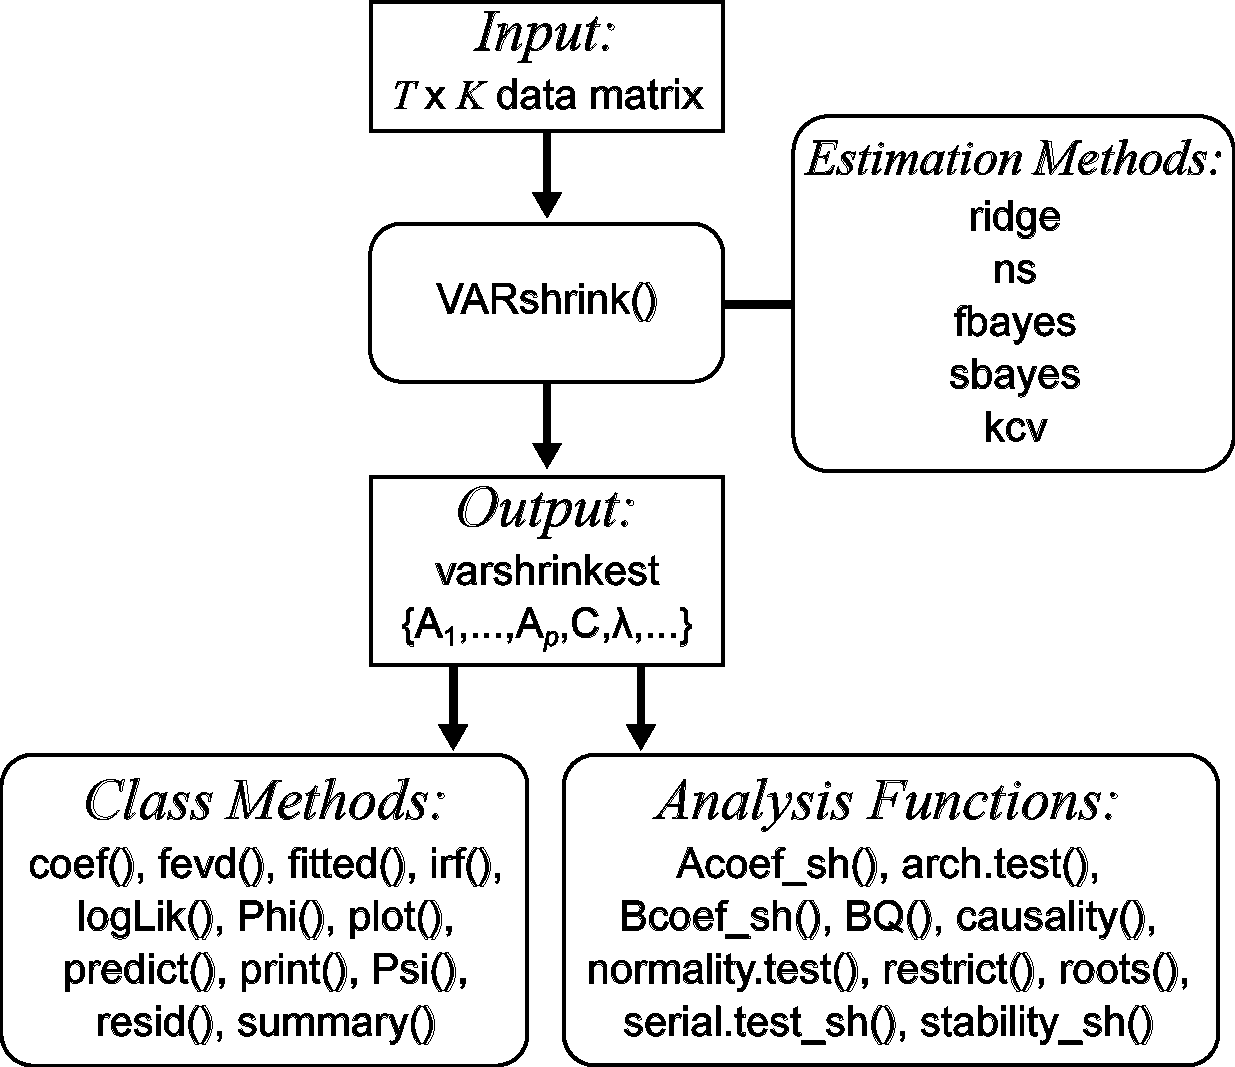
\includegraphics[width=0.6\linewidth,alt={Systematic diagram of the VARshrink package, consisting of the inputs and outputs of the main function, together with class methods and analysis functions.}]{figures/software_architecture} 

}

\caption{Systematic diagram of the VARshrink package.}\label{fig:architecture}
\end{figure}

The class \texttt{varshrinkest} inherits from the class \texttt{varest} in the \CRANpkg{vars} package. Consequently, all class methods available for \texttt{varest} can also be applied to \texttt{varshrinkest}, such as \texttt{fevd()}, \texttt{Phi()}, and \texttt{plot()}.
We also note that the classes \texttt{varshrinkest},
\texttt{varshirf}, and \texttt{varshsum} inherit from \texttt{varest},
\texttt{varirf}, and \texttt{varsum}, respectively, in the \CRANpkg{vars} package.

\begin{table}
\centering
\caption{\label{tab:methods-pdf}Structure of the VARshrink package.}
\centering
\fontsize{9}{11}\selectfont
\begin{tabular}[t]{>{\raggedright\arraybackslash}p{7em}|>{\raggedright\arraybackslash}p{8em}|>{\raggedright\arraybackslash}p{9em}|>{\raggedright\arraybackslash}p{12em}}
\hline
Function or method & Class & Class methods & Analysis functions for class\\
\hline
VARshrink & varshrinkest, varest & coef, fevd, fitted, irf, logLik, Phi, plot, predict, print, Psi, resid, summary & Acoef\_sh, arch.test, Bcoef\_sh, BQ, causality, normality.test, restrict, roots, serial.test\_sh, stability\_sh\\
\hline
fevd & varfevd & plot, print & \\
\hline
irf & varshirf, varirf & plot, print & \\
\hline
predict & varprd & plot, print & fanchart\\
\hline
summary & varshsum, varsum & print & \\
\hline
arch.test & varcheck & plot, print & \\
\hline
normality.test & varcheck & plot, print & \\
\hline
serial.test\_sh & varcheck & plot, print & \\
\hline
stability\_sh & varstabil & plot, print & \\
\hline
\end{tabular}
\end{table}

The class method \texttt{irf.varshrinkest()} retains the interface and identification options of \texttt{vars::irf()}. For shrinkage estimators, confidence intervals are obtained via bootstrap procedures that require repeatedly refitting the model. In contrast, when the full Bayesian method is fitted with \texttt{store\_mcmc\ =\ TRUE}, \texttt{irf()} can construct Bayesian credible intervals directly from the stored MCMC draws of the VAR coefficients, avoiding the computational cost of bootstrap-based interval estimation.

\subsection{Main function}\label{main-function}

We provide a common \textbf{R} function interface \texttt{VARshrink()}
for running the estimation methods, which is defined by

\begin{verbatim}
VARshrink(y, p = 1, type = c("const", "trend", "both", "none"),
   season = NULL, exogen = NULL, method = c("ridge", "ns",
   "fbayes", "sbayes", "kcv", "ols"), lambda = NULL, lambda_var = NULL,
   dof = Inf, ...)
\end{verbatim}

The input arguments are described as follows.

\begin{itemize}
\item
  \texttt{y}: A \(T \times K\) matrix of endogenous variables
\item
  \texttt{p}: Integer for the lag order
\item
  \texttt{type}: Type of deterministic regressors to include.

  \begin{enumerate}
  \def\labelenumi{\arabic{enumi}.}
  \tightlist
  \item
    ``const'' - the constant: \(\mathbf{d}_t = 1\).
  \item
    ``trend'' - the trend: \(\mathbf{d}_t = t\).
  \item
    ``both'' - both the constant and the trend:
    \(\mathbf{d}_t = (t, 1)^\top\).
  \item
    ``none'' - no deterministic regressors.
  \end{enumerate}
\item
  \texttt{season}: An integer value of frequency for inclusion of centered
  seasonal dummy variables.
\item
  \texttt{exogen}: A \(T \times L\) matrix of exogenous variables.
\item
  \texttt{method}:

  \begin{enumerate}
  \def\labelenumi{\arabic{enumi}.}
  \tightlist
  \item
    ``ridge'' - multivariate ridge regression \citep{Hoerl70, Golub79, Ripley18}.
  \item
    ``ns'' - a Stein-type nonparametric shrinkage method \citep{Schafer05b, Rhein07c, Schafer17}.
  \item
    ``fbayes'' - a full Bayesian shrinkage method using noninformative
    priors \citep{Sun04, Ni05}.
  \item
    ``sbayes'' - a semiparametric Bayesian shrinkage method using
    parameterized cross-validation \citep{LeeChoiKim2016}.
  \item
    ``kcv'' - a semiparametric Bayesian shrinkage method using K-fold
    cross-validation \citep{LeeChoiKim2016}.
  \item
    ``ols'' - ordinary least squares estimation, calling \texttt{vars::VAR()}.
  \end{enumerate}
\item
  \texttt{lambda}, \texttt{lambda\_var}: Shrinkage parameter value(s). Use of this
  parameter is slightly different for each method: the same value does
  not imply the same shrinkage estimates. See the description in the
  previous section for the use of shrinkage parameters in each
  method.
\item
  \texttt{dof}: Degree of freedom of multivariate t-distribution for
  noise. Valid only for \texttt{method\ =\ "fbayes"} and
  \texttt{method\ =\ "sbayes"}. \texttt{dof\ =\ Inf} means multivariate normal
  distribution.
\item
  \texttt{...}: Additional method-specific options, including
  \texttt{store\_mcmc\ =\ TRUE} for retaining MCMC draws from the full Bayesian
  method.
\end{itemize}

\subsection{Sample code snippets analysis}\label{sample-code-snippets-analysis}

Simulated time series data of length \(T=100\) were
generated from a VAR model with order \(p=1\) and dimension \(K=2\), assuming
multivariate normal noise. The model parameters were set as
\(\mathbf{A}_1 = 0.5\mathbf{I}_2\),
\(\mathbf{C}=(0.2, 0.7)^\top\), and
\(\mathbf{\Sigma} = 0.1^2\mathbf{I}_2\), as follows:

\begin{verbatim}
set.seed(1000)
myCoef <- list(A = list(matrix(c(0.5, 0, 0, 0.5), 2, 2)), c = c(0.2, 0.7))
myModel <- list(Coef = myCoef, Sigma = diag(0.1^2, 2), dof = Inf)
Y <- simVARmodel(numT = 100, model = myModel, burnin = 10)
resu_estim <- list()
\end{verbatim}

The multivariate ridge regression for VAR
models can be performed as follows. The output displays all the candidate
\texttt{lambda} values along with their corresponding generalized cross-validation (GCV) scores \citep{Golub79}. The VAR parameters are then estimated using the lambda value that yields the minimum GCV score.

\begin{verbatim}
resu_estim$`Ridge regression` <-
  VARshrink(Y, p = 1, type = "const", method = "ridge", lambda = NULL)
resu_estim$`Ridge regression`
\end{verbatim}

\begin{verbatim}
#> 
#> VAR Shrinkage Estimation Results:
#> ================================= 
#> 
#> Estimated coefficients for equation y1: 
#> ======================================= 
#> Call:
#> y1 = y1.l1 + y2.l1 + const 
#> 
#>      y1.l1      y2.l1      const 
#> 0.61424699 0.07318362 0.05264740 
#> 
#> 
#> Estimated coefficients for equation y2: 
#> ======================================= 
#> Call:
#> y2 = y1.l1 + y2.l1 + const 
#> 
#>     y1.l1     y2.l1     const 
#> 0.1195550 0.3254618 0.9055450 
#> 
#> 
#> lambda: 5e-04 (estimated: TRUE) 
#> GCV:  0.0186
\end{verbatim}

The \texttt{summary()} method reports the estimated coefficient matrices,
shrinkage parameters, noise covariance matrix, and method-specific fitting
information.

After estimation, the fitted object can be used in a standard VAR workflow
for diagnostic checking, forecasting, impulse response analysis, and
forecast error variance decomposition. The returned objects have their own
\texttt{plot()} methods.

\begin{verbatim}
fit_ridge <- resu_estim$`Ridge regression`

plot(fit_ridge)

diagnostics <- list(
  serial = serial.test_sh(fit_ridge),
  arch = arch.test(fit_ridge),
  normality = normality.test(fit_ridge),
  stability = stability_sh(fit_ridge)
)

plot(predict(fit_ridge, n.ahead = 5), names = "y1")

plot(irf(fit_ridge, impulse = "y1", response = "y2", n.ahead = 10,
         ortho = TRUE, boot = TRUE))

plot(fevd(fit_ridge, n.ahead = 10))
\end{verbatim}

The class methods \texttt{AIC()} and \texttt{BIC()} can be used to compute the Akaike Information Criterion (AIC) and the Bayesian Information Criterion (BIC) as follows:

\begin{verbatim}
c(AIC = AIC(resu_estim$`Ridge regression`),
  BIC = BIC(resu_estim$`Ridge regression`))
\end{verbatim}

\begin{verbatim}
#>       AIC       BIC 
#> -366.2358 -351.5082
\end{verbatim}

An OLS and the other shrinkage estimation methods (``ns'',
``fbayes'', ``sbayes'', and ``kcv'') can be run similarly. For ``ns'',
``sbayes'', and ``kcv'', if the input arguments \texttt{lambda} and \texttt{lambda\_var}
are set to \texttt{NULL}, the shrinkage parameters \(\lambda\) and \(\lambda_v\)
are determined automatically.
For ``fbayes'', ``sbayes'', and ``kcv'', the degree of freedom \(\nu\) of the multivariate \(t\)-distribution for noise can either be set to a fixed value or estimated automatically by specifying the argument \texttt{dof}.
For ``fbayes'', ``sbayes'', and ``kcv'', \texttt{prior\_type} can be set to either \texttt{"CJ"} or \texttt{"NCJ"} corresponding to conjugate and non-conjugate prior distributions, respectively.

\begin{verbatim}
resu_estim$`Ordinary least squares` <-
  VARshrink(Y, p = 1, type = "const", method = "ols")
resu_estim$`Nonparametric shrinkage` <-
  VARshrink(Y, p = 1, type = "none", method = "ns", lambda = NULL,
            lambda_var = NULL)
resu_estim$`Full Bayes (fixed dof)` <-
  VARshrink(Y, p = 1, type = "const", method = "fbayes", dof = 6,
            prior_type = "NCJ", burnincycle = 1000, mcmccycle = 2000,
            store_mcmc = TRUE)
resu_estim$`Full Bayes (estim dof)` <-
  VARshrink(Y, p = 1, type = "const", method = "fbayes", dof = NULL,
            prior_type = "NCJ", burnincycle = 1000, mcmccycle = 2000,
            store_mcmc = TRUE)
resu_estim$`Semi Bayes (fixed dof)` <-
  VARshrink(Y, p = 1, type = "const", method = "sbayes", dof = 6,
            prior_type = "NCJ", lambda = NULL, lambda_var = NULL, num_folds = 5)
resu_estim$`Semi Bayes (estim dof)` <-
  VARshrink(Y, p = 1, type = "const", method = "sbayes", dof = NULL,
            prior_type = "NCJ", lambda = NULL, lambda_var = NULL, num_folds = 5)
resu_estim$`K-fold CV (fixed dof)` <-
  VARshrink(Y, p = 1, type = "const", method = "kcv", dof = 6,
            prior_type = "NCJ", lambda = NULL, lambda_var = NULL, num_folds = 5)
resu_estim$`K-fold CV (estim dof)` <-
  VARshrink(Y, p = 1, type = "const", method = "kcv", dof = NULL,
            prior_type = "NCJ", lambda = NULL, lambda_var = NULL, num_folds = 5)
\end{verbatim}

\section{Illustrative examples}\label{illustrative-examples}

\subsection{Benchmark data}\label{benchmark-data}

The Canada dataset is a benchmark macroeconomic dataset included in the \CRANpkg{vars} package. It contains four time series variables: employment (\texttt{e}), labor productivity (\texttt{prod}), real wage (\texttt{rw}), and unemployment rate (\texttt{U}), with 84 observations. We differenced the data to remove the trend, resulting in \(T=83\). Figure \ref{fig:diffCanada} shows the differenced series.

\begin{figure}

{\centering \includegraphics[width=0.7\linewidth,alt={A visualization of the benchmark dataset obtained by differencing the Canada time series from the vars package, consisting of four variables labeled e, prod, rw, and U.}]{RJ-2026-042_files/figure-latex/diffCanada-1} 

}

\caption{Benchmark dataset obtained by differencing the Canada time series from the vars package.}\label{fig:diffCanada}
\end{figure}

We illustrate the use of AIC and BIC for comparing VAR models with
varying lag order \(p=1,2,3\). OLS is included as a baseline, shrinkage
parameters were selected automatically for the shrinkage methods, and
for ``fbayes'', ``sbayes'', and ``kcv'', the \texttt{dof} argument was set to \texttt{NULL}.
Table \ref{tab:modelcomp-pdf} shows that, using the NS method, AIC attains its minimum at \(p=3\), whereas BIC attains its minimum at \(p=2\).

\begin{table}
\centering
\caption{\label{tab:modelcomp-pdf}Information criteria (AIC and BIC) for model comparison.}
\centering
\fontsize{9}{11}\selectfont
\begin{tabular}[t]{l|r|r|r|r|r|r}
\hline
  & AIC.p=1 & BIC.p=1 & AIC.p=2 & BIC.p=2 & AIC.p=3 & BIC.p=3\\
\hline
Ordinary least squares & 467.6 & 515.7 & 444.2 & 530.4 & 452.3 & 576.2\\
\hline
Ridge regression & 465.8 & 504.6 & 442.9 & 509.3 & 445.3 & 525.9\\
\hline
Nonparametric shrinkage & 454.5 & 478.9 & 426.6 & 471.4 & 422.5 & 485.4\\
\hline
Full Bayes & 457.0 & 497.2 & 444.2 & 508.2 & 445.3 & 523.8\\
\hline
Semi Bayes & 533.2 & 577.5 & 574.1 & 656.1 & 475.0 & 553.4\\
\hline
K-fold CV & 495.7 & 538.2 & 466.2 & 525.4 & 472.9 & 538.1\\
\hline
\end{tabular}
\end{table}

The parameters estimated by the NS method with \(p=2\) can be further analyzed using the class methods and functions listed in Table \ref{tab:methods-pdf}. For example, a test for serially correlated errors and an ARCH test can be performed as follows:

\begin{verbatim}
fitted_Canada <- VARshrink(Y, p = 2, type = "none", method = "ns")
serial.test(fitted_Canada)
\end{verbatim}

\begin{verbatim}
#> 
#>  Portmanteau Test (asymptotic)
#> 
#> data:  Residuals of VAR object fitted_Canada
#> Chi-squared = 176.31, df = 228, p-value = 0.9953
\end{verbatim}

\begin{verbatim}
arch.test(fitted_Canada)
\end{verbatim}

\begin{verbatim}
#> 
#>  ARCH (multivariate)
#> 
#> data:  Residuals of VAR object fitted_Canada
#> Chi-squared = 508.04, df = 500, p-value = 0.3921
\end{verbatim}

We can inspect the summary results to assess the statistical significance of each covariate affecting the unemployment rate through the model coefficients:

\begin{verbatim}
summary_Canada <- summary(fitted_Canada)
print(summary_Canada$varresult[["U"]])
\end{verbatim}

\begin{verbatim}
#> 
#> Call:
#> VARshrink(y = Y, p = 2, type = "none", method = "ns")
#> 
#> Residuals:
#>      Min       1Q   Median       3Q      Max 
#> -0.84400 -0.16754 -0.00281  0.16971  0.72526 
#> 
#> Coefficients:
#>         Estimate Std. Error t value Pr(>|t|)    
#> e.l1    -0.36506    0.03356 -10.877  < 2e-16 ***
#> prod.l1 -0.13332    0.03502  -3.807 0.000283 ***
#> rw.l1    0.03840    0.02940   1.306 0.195426    
#> U.l1     0.07101    0.03193   2.224 0.029098 *  
#> e.l2     0.01561    0.03265   0.478 0.633932    
#> prod.l2 -0.04137    0.03533  -1.171 0.245312    
#> rw.l2    0.09894    0.02930   3.377 0.001157 ** 
#> U.l2    -0.11933    0.03161  -3.775 0.000314 ***
#> ---
#> Signif. codes:  0 '***' 0.001 '**' 0.01 '*' 0.05 '.' 0.1 ' ' 1
#> 
#> Residual standard error: 0.2937 on 76.32037 degrees of freedom
#> Multiple R-squared:  0.5625, Adjusted R-squared:  0.5414 
#> F-statistic: 26.67 on 3.679632 and 76.32037 DF,  p-value: 2.873e-13
\end{verbatim}

It is worthwhile to examine the correlations among the noise variables to evaluate
concurrent relationships between the time series variables within the residuals:

\begin{verbatim}
print(round(summary_Canada$corres, 3))
\end{verbatim}

\begin{verbatim}
#>           e   prod     rw      U
#> e     1.000 -0.070 -0.039 -0.687
#> prod -0.070  1.000  0.086  0.018
#> rw   -0.039  0.086  1.000  0.207
#> U    -0.687  0.018  0.207  1.000
\end{verbatim}

Time series forecasting can be performed, as illustrated in Figure \ref{fig:pred}.

\begin{verbatim}
plot(predict(fitted_Canada), names = "U")
\end{verbatim}

\begin{figure}

{\centering \includegraphics[width=0.7\linewidth,alt={10-step-ahead forecast of the differenced Canada time series using the VAR model estimated via the NS method with lag order p=2.}]{RJ-2026-042_files/figure-latex/pred-1} 

}

\caption{10-step-ahead forecast of the differenced Canada time series using the VAR model estimated via the NS method with lag order $p=2$.}\label{fig:pred}
\end{figure}

Impulse responses can be computed from the same fitted object.

\pandocbounded{\includegraphics[keepaspectratio]{RJ-2026-042_files/RJ-2026-042_files/figure-latex/structural-Canada-1.pdf}}

\subsection{Comparative simulation}\label{comparative-simulation}

We generated multivariate time series data of length
\(T = 20, 40, 80, 160\) from \(K = 20\) dimensional VAR models of order
\(p = 1\). Note that for \(T = 20\), the sample size
\(N = T - p = 19\) is smaller than the dimensionality \(K = 20\).
The VAR coefficient matrix \(\mathbf{A}_1\) was specified with
diagonal entries of 0.6 and zeros elsewhere, except for
\(K\) entries randomly selected from the lower triangular part of the
matrix. The nonzero off-diagonal entries were drawn uniformly at random
from the intervals \([-1, -0.2]\) and \([0.2, 1]\).
Since the coefficient matrix is lower triangular, the diagonal entries determine its eigenvalues, which lead to weak stationarity \citep{Hamilton94, Tsay05}.
The noise \(\boldsymbol\epsilon_t\) was randomly sampled from the multivariate normal distribution whose covariance matrix has diagonal entries of 1 and off-diagonal entries of 0.5.
The experiments were repeated 50 times. We compared the four shrinkage
methods and, when \(T-p>K\), the OLS baseline. The sum of squared errors
(SSEs) of the estimated VAR coefficients was used as a measure of
parameter estimation accuracy.
The summary of the coefficient SSEs is shown in
Figure \ref{fig:comparisons-K20}. The figure shows that
the full Bayesian and semiparametric Bayesian methods produced accurate
estimates with low SSEs, particularly for larger values of \(T\), as they
correctly incorporated correlations among the noise variables.

\begin{figure}
\includegraphics[width=1\linewidth,alt={Comparison of mean SSEs across the four shrinkage methods and the OLS, with sample size increasing from 20 to 160.}]{RJ-2026-042_files/figure-latex/comparisons-K20-1} \caption{Comparison of mean SSEs across the four shrinkage methods and the OLS.}\label{fig:comparisons-K20}
\end{figure}

Figure \ref{fig:comparisons-K20-msfe} presents the out-of-sample
forecasting performance of the shrinkage methods and the OLS baseline
when estimable. Figure
\ref{fig:comparisons-K20-time} presents the computational costs of the
same methods as a function of the sample size. The full Bayesian method
required the largest computational cost, indicating that computationally
efficient alternative methods are needed for high-dimensional time series
analysis.

\begin{figure}
\includegraphics[width=1\linewidth,alt={Comparison of 10-step out-of-sample mean squared forecast errors across the four shrinkage methods and the OLS baseline when estimable, with sample size increasing from 20 to 160.}]{RJ-2026-042_files/figure-latex/comparisons-K20-msfe-1} \caption{Comparison of 10-step out-of-sample MSFEs across the four shrinkage methods and the OLS baseline when estimable.}\label{fig:comparisons-K20-msfe}
\end{figure}

\begin{figure}

{\centering \includegraphics[width=0.8\linewidth,alt={Comparison of average estimation times across the four shrinkage methods and the OLS baseline when estimable as sample size increases from 20 to 160, shown on a linear y-axis.}]{RJ-2026-042_files/figure-latex/comparisons-K20-time-1} 

}

\caption{Comparison of computational costs across the four shrinkage methods and the OLS baseline when estimable as sample size increases.}\label{fig:comparisons-K20-time}
\end{figure}

To assess scalability with respect to the number of VAR coefficients, we
also varied the dimension \(K\) while holding \(T=160\) and \(p=1\) fixed.
The number of autoregressive coefficients is \(K^2p\).
As shown in Figure \ref{fig:comparisons-param-time}, computational costs increase much more rapidly with the number of VAR coefficients than with the sample size.

\begin{figure}

{\centering \includegraphics[width=0.8\linewidth,alt={Comparison of average estimation times across the four shrinkage methods and the OLS baseline as the number of VAR coefficients increases, shown on a linear y-axis.}]{RJ-2026-042_files/figure-latex/comparisons-param-time-1} 

}

\caption{Comparison of computational costs across the four shrinkage methods and the OLS baseline as the number of VAR coefficients increases.}\label{fig:comparisons-param-time}
\end{figure}

\section{Discussion}\label{discussion}

The \textbf{R} ecosystem for multivariate time series has become increasingly
specialized, as reflected in the CRAN Time Series Task View
\citep{Hyndman2026cran}. Packages such as \CRANpkg{vars} and \CRANpkg{MTS} provide
established tools for VAR estimation, forecasting, and post-estimation
analysis. Other packages focus on modern extensions: \CRANpkg{BigVAR}
and \CRANpkg{bigtime} emphasize penalized estimation for large
multivariate systems \citep{Nicholson2026BigVAR, Wilms2023bigtime}, while
\CRANpkg{BVAR}, \CRANpkg{bayesianVARs}, \CRANpkg{bvarsv}, and
\CRANpkg{bvartools} support Bayesian workflows involving hierarchical
prior selection, MCMC estimation, and stochastic volatility
\citep{Giannone2015prior, KuschnigVashold2021BVAR, Gruber2026bayesianVARs, Primiceri2005timevarying, Krueger2015bvarsv, Mohr2024bvartools}.
For structural Bayesian VARs, \CRANpkg{bsvarSIGNs} provides tools for
sign, zero, and narrative restrictions \citep{WangWozniak2025bsvarSIGNs}.

\CRANpkg{VARshrink} is designed to complement these packages by bringing
an OLS baseline and several shrinkage estimators into a common interface
compatible with the widely used \CRANpkg{vars} workflow. It currently
includes multivariate ridge regression \citep{Hoerl70, Golub79}, a Stein-type
nonparametric shrinkage method \citep{Rhein07c}, fully Bayesian methods with
natural conjugate and non-conjugate priors \citep{Ni05}, and semiparametric
Bayesian methods \citep{LeeChoiKim2016}. This design allows users to compare
OLS and alternative shrinkage estimators while retaining familiar tools for
coefficient extraction, fitted values, residuals, forecasting, impulse
responses, forecast error variance decompositions, diagnostic tests, and
visualization.

The package is intended for applied researchers, students, and analysts
who use the \CRANpkg{vars} workflow but need more stable estimation than
ordinary least squares can provide. Such settings arise when the number
of variables is large relative to the number of observations, as in
macroeconomic forecasting, financial systems, gene regulatory network
analysis, and dynamic brain connectivity analysis
\citep{Harrison03, Rhein07c, Banbura10}. In these applications, shrinkage is
useful not only for forecasting but also for stabilizing coefficient
estimates used to study dynamic relationships, partial correlation
structures, impulse responses, and forecast error variance
decompositions.

The structural analysis tools in \CRANpkg{VARshrink} come from this
interoperability with \CRANpkg{vars}. Because \texttt{varshrinkest} objects
inherit from \texttt{varest}, users can apply familiar post-estimation tools
from \CRANpkg{vars}. For impulse responses, uncertainty calculation is
estimator-specific: bootstrap re-estimation can be costly for shrinkage
estimators, whereas stored MCMC draws can be used by \texttt{irf()} to form
Bayesian credible intervals when the full Bayesian method is fitted with
\texttt{store\_mcmc\ =\ TRUE}.
Users whose main goal is advanced structural identification, stochastic
volatility, or sign, zero, and narrative restrictions may therefore
prefer packages designed specifically for those purposes.

Several limitations remain. \CRANpkg{VARshrink} does not yet implement
the full range of modern Bayesian shrinkage priors, such as
Minnesota-type, global-local, or hierarchical priors used in
macroeconomic forecasting \citep{Doan84, Litterman86, KastnerHuber2017, Giannone2015prior}.
It also inherits structural identification from \CRANpkg{vars} rather
than developing a separate structural VAR framework. Finally, fully
Bayesian estimation provides richer posterior information but is more
computationally expensive than ridge or nonparametric shrinkage,
especially as the number of variables grows. These limitations define
the current scope of the package and suggest future extensions, including
additional prior structures, structured penalties, and closer integration
with modern structural VAR workflows.

\section{Conclusions}\label{conclusions}

Shrinkage methods are useful for VAR models when the number of
parameters is large relative to the sample size. The \textbf{R} package
\CRANpkg{VARshrink} provides an OLS baseline and ridge, nonparametric,
fully Bayesian, and semiparametric shrinkage estimators through a unified
interface connected to the familiar \CRANpkg{vars} class system. This
allows users to compare OLS with shrinkage methods and then apply standard
VAR tools for forecasting,
visualization, diagnostics, impulse responses, and forecast error
variance decompositions.

\CRANpkg{VARshrink} complements specialized software for penalized
forecasting, Bayesian prior selection, stochastic volatility, and
structural identification. Its main role is to provide a common workflow
for stable VAR coefficient estimation in high-dimensional settings.
Future development can extend this framework with additional prior
structures, structured penalties, and richer structural analysis tools
while preserving compatibility with established VAR workflows in \textbf{R}.

\section*{Computational details}\label{computational-details}
\addcontentsline{toc}{section}{Computational details}

The results in this manuscript were obtained using \textbf{R} 4.5.3 and \CRANpkg{VARshrink} 0.5.0 on a MacBook running macOS 26.3.1, equipped with an Apple M4 Pro CPU and 24GB of memory.

\section*{Supplementary materials}\label{supplementary-materials}
\addcontentsline{toc}{section}{Supplementary materials}

varshrink-rjournal.R: R code to reproduce all the results in the manuscript.

\section*{Acknowledgements}\label{acknowledgements}
\addcontentsline{toc}{section}{Acknowledgements}

This work was supported by the National Research Foundation of Korea (NRF) grants funded by the Ministry of Science and ICT (MSIT) (RS-2024-00336424, RS-2024-00358572) and the Ministry of Education (MOE) (RS-2025-25415913) of the Republic of Korea. N. Lee was supported by the Regional Innovation System \& Education (RISE) program through the Gangwon RISE Center funded by the MOE and the Gangwon State (G.S.), Republic of Korea (2026-RISE-10-002).

\section*{Conflict of interest}\label{conflict-of-interest}
\addcontentsline{toc}{section}{Conflict of interest}

The authors have no competing interests to declare that are relevant to the content of this article.

\section*{Data availability}\label{data-availability}
\addcontentsline{toc}{section}{Data availability}

The Canada dataset was deposited by other researchers and is available in the \textbf{R} package \CRANpkg{vars} at the CRAN repository, \url{https://CRAN.R-project.org/package=vars}.

\bibliography{varshrink-rjournal.bib}

\address{%
Namgil Lee\\
Kangwon National University\\%
Department of Information Statistics, Kangwon National University, Chuncheon, Gangwon 24341, Republic of Korea\\ Bionsight, Chuncheon, Gangwon 24341, Republic of Korea\\
%
%
\textit{ORCiD: \href{https://orcid.org/0000-0003-0593-9028}{0000-0003-0593-9028}}\\%
\href{mailto:namgil.lee@kangwon.ac.kr}{\nolinkurl{namgil.lee@kangwon.ac.kr}}%
}

\address{%
Sung-Ho Kim\\
KAIST\\%
Department of Mathematical Sciences, KAIST, Daejeon 34141, Republic of Korea\\
%
%
%
\href{mailto:sung-ho.kim@kaist.edu}{\nolinkurl{sung-ho.kim@kaist.edu}}%
}
